\section{量化索引的压缩}
\label{sec:quant-index-coding}

到目前为止，每个索引都按定长写出，$N$个点用$\log_2N$个比特。可是索引并不等可能：Laplace读数的四点Lloyd--Max量化器中，内侧两个区间各占约$40\%$，外侧两个各占约$10\%$。上一章说过，概率不均匀的离散信源可以用变长码缩短平均长度。量化索引正是这样一个离散信源。

\paragraph{固定量化器后的索引编码}
量化器固定后，索引$J=\alpha(X)$的分布由式~\eqref{eq:quant-index-pmf}给出。对$J$使用第~\ref{chap:lossless-coding}章的前缀码，接收端能精确恢复$J$，再由解码器报出同一个重构值。重构结果、从而平均失真都没有改变，改变的只是平均描述长度。由上一章的平均码长界，最好的前缀码满足
\begin{equation}
 H(J)\leq\bar{\ell}<H(J)+1 ,
 \label{eq:quant-index-length-bound}
\end{equation}
其中$\bar{\ell}=\sum_jp_j\ell(j)$是平均码长，$H(J)$是索引的熵。

以第~\ref{sec:quant-nonuniform}节得到的四点不动点量化器为例。外侧区间$\lvert X\rvert\geq1.5936$的概率是$\mathrm{e}^{-1.5936}=0.2032$，两侧平分，于是索引的分布为
\[
 (p_1,p_2,p_3,p_4)=(0.1016,\ 0.3984,\ 0.3984,\ 0.1016) .
\]
它的熵为
\[
 H(J)=-2\bigl(0.1016\log_20.1016+0.3984\log_20.3984\bigr)=1.728\ \text{bit} .
\]

用Huffman编码构造码树：先合并两个最小的概率$0.1016$与$0.1016$，得$0.2032$；再与一个$0.3984$合并，得$0.6016$；最后与另一个$0.3984$合并。码长依次为$1,2,3,3$，平均码长为
\[
 \bar{\ell}=0.3984\times1+0.3984\times2+0.1016\times3\times2=1.805\ \text{bit} .
\]
图~\ref{fig:quant-index-huffman}画出了这棵码树。与定长的$2$个比特相比，平均每个读数省下约$0.2$个比特，平均失真仍是$0.3524$。若把两个读数的索引组成一对再编码，每读数的平均码长不超过$H(J)+\tfrac12$；块越长，越接近$1.728$。

\begin{BookInlineFigure}
 \centering
 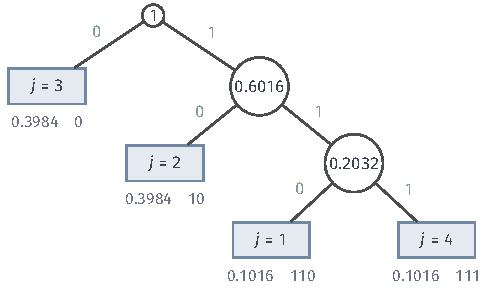
\includegraphics[width=83.4mm]{figures/07-probability/05-source-coding/tikz/quant-index-huffman/figure.pdf}
 \caption{$\operatorname{Laplace}(0,1)$四点Lloyd--Max量化器索引的Huffman码树。叶结点下方是区间概率与码字，内部结点标出合并后的概率，绿色数字是分支标号。平均码长为$1.805$ bit，索引的熵为$1.728$ bit。}
 \label{fig:quant-index-huffman}
\end{BookInlineFigure}

\paragraph{均匀量化配合熵编码}
变长描述还改变了对有限范围的要求。定长索引必须事先限定点数，因而必须规定表示范围，范围外的读数产生过载误差。变长描述却可以使用无穷多个区间：取步长为$\Delta$、零为重构值的均匀刻度，
\begin{equation}
 Q_{\Delta}(x)=\Delta\Bigl\lfloor\frac{x}{\Delta}+\frac12\Bigr\rfloor ,
 \label{eq:quant-midtread}
\end{equation}
它把$[(k-\frac12)\Delta,(k+\frac12)\Delta)$映到$k\Delta$，$k$取遍全体整数。远处的区间概率极小，给它们很长的码字，对平均长度几乎没有影响，而误差始终不超过$\Delta/2$。

索引集合可数无穷时，Huffman编码的构造不再直接适用，但长度为$\ell(k)=\lceil-\log_2p_k\rceil$的前缀码仍然存在：这些长度满足$\sum_k2^{-\ell(k)}\leq\sum_kp_k=1$，按长度从短到长依次在码树上分配码字即可，平均长度小于$H(J)+1$。所以对均匀量化配合熵编码，描述资源由索引的熵衡量。

\paragraph{索引熵与微分熵}
步长很小时，索引的熵可以用读数的微分熵近似。回顾第~\ref{chap:information-measures}章，具有密度$f$的读数的微分熵是
\[
 h(X)=-\int f(x)\log_2f(x)\,\mathrm{d}x .
\]
对Laplace读数，$-\log_2f(x)=1+\lvert x\rvert\log_2\mathrm{e}$，又$\mathbb{E}\lvert X\rvert=1$，所以
\[
 h(X)=1+\log_2\mathrm{e}=\log_2(2\mathrm{e})\approx2.443\ \text{bit} .
\]

若密度在每个长度为$\Delta$的区间内变化不大，区间概率近似为$p_k\approx f(k\Delta)\Delta$。代入索引的熵，
\[
 H(J)=-\sum_kp_k\log_2p_k\approx-\sum_kp_k\log_2f(k\Delta)-\log_2\Delta .
\]
第一项是$-\log_2f$在区间代表点上按区间概率加权的和，在$\Delta\to0$时趋于积分$h(X)$。于是
\begin{equation}
 H\bigl(Q_{\Delta}(X)\bigr)\approx h(X)-\log_2\Delta .
 \label{eq:quant-index-entropy-highres}
\end{equation}
步长减半，索引的熵增加一个比特，相当于每个区间分成两半、需要多问一个是非题。在密度足够规则（例如Riemann可积且$H(Q_1(X))$有限）时，式~\eqref{eq:quant-index-entropy-highres}两边之差在$\Delta\to0$时趋于零，证明可查阅~\scite{math-cover2006information}。

\begin{BookInlineFigure}
 \centering
 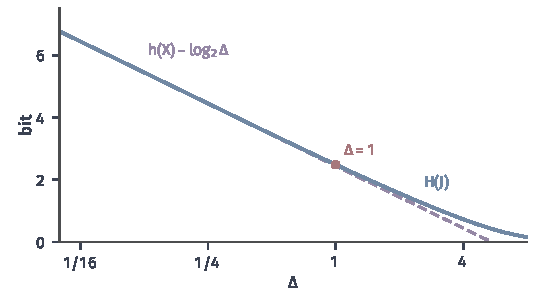
\includegraphics[width=92mm]{figures/07-probability/05-source-coding/matplotlib/quant-entropy-step/figure.pdf}
 \caption{$\operatorname{Laplace}(0,1)$读数经步长为$\Delta$的无穷均匀量化器~\eqref{eq:quant-midtread}后索引的熵。蓝线为精确值，紫色虚线为近似$h(X)-\log_2\Delta$，$h(X)=\log_2(2\mathrm{e})$；横轴为对数刻度。红点为$\Delta=1$，精确值$2.484$ bit，近似值$2.443$ bit。}
 \label{fig:quant-index-entropy}
\end{BookInlineFigure}

图~\ref{fig:quant-index-entropy}比较两者。$\Delta=1$时精确值为$2.484$ bit，近似值为$2.443$ bit，已经相当接近；步长再小，两条曲线几乎重合。步长大到与分布的尺度相当时近似失效：$\Delta=4$时近似值为负，而熵不可能为负，此时中央区间的概率已达$0.865$。

\paragraph{比较时固定相同的资源}
现在可以在相同的平均描述长度下比较不同方案。图~\ref{fig:quant-operational}画出Laplace读数的平均失真随每读数比特数的变化。黄线和绿线是定长索引的最好均匀量化器与Lloyd--Max量化器，横坐标为$\log_2N$；蓝线是无穷均匀量化器配合熵编码，横坐标为索引的熵$H(J)$；红点是四点Lloyd--Max量化器配合熵编码。

\begin{BookInlineFigure}
 \centering
 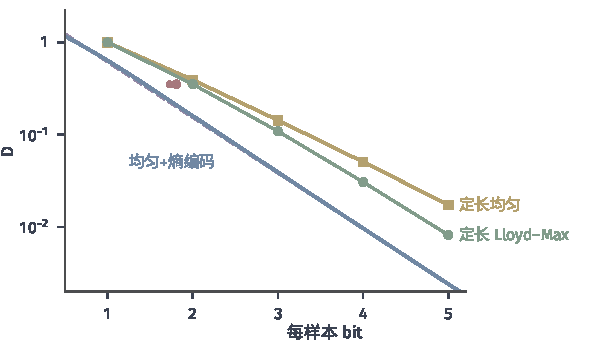
\includegraphics[width=100mm]{figures/07-probability/05-source-coding/matplotlib/quant-operational/figure.pdf}
 \caption{$\operatorname{Laplace}(0,1)$读数的平均失真与每读数比特数（纵轴为对数刻度）。黄色方块：定长索引的最好均匀量化器，$N=2,4,\dots,32$；绿色圆点：定长索引的Lloyd--Max量化器；蓝线：无穷均匀量化器配合熵编码，横坐标为索引的熵；紫色虚线：高分辨率公式$\frac{(2\mathrm{e})^{2}}{12}2^{-2R}$，与蓝线几乎重合；红点：四点Lloyd--Max量化器配合Huffman码（$1.805$ bit）与理想码长（$1.728$ bit）。}
 \label{fig:quant-operational}
\end{BookInlineFigure}

图中的排序很清楚。在约$1.8$ bit处，四点Lloyd--Max量化器加Huffman码的失真是$0.352$，而步长约为$1.66$的均匀量化器加熵编码，失真只有$0.212$。在定长$3$ bit处，Lloyd--Max量化器的失真是$0.109$；均匀量化器加熵编码只用约$2.5$ bit（$\Delta=1$）就达到$0.081$。分布越不均匀、尾部越重，这种差距越明显。

蓝线在比特数较大时几乎是一条直线，斜率对应“每多一个比特，失真降为四分之一”。这可以由两个近似合起来解释：范围内的误差近似为$\Delta^{2}/12$（第~\ref{sec:quant-granular-overload}节），索引熵近似为式~\eqref{eq:quant-index-entropy-highres}。消去$\Delta$，得到平均描述长度为$R$时
\begin{equation}
 D\approx\frac{1}{12}\,2^{2h(X)}\,2^{-2R} .
 \label{eq:quant-highres-ec}
\end{equation}
这是一个高分辨率近似，紫色虚线就是它；在$R$较小时它不再可靠。

\paragraph{把码长写进目标}
上面的方案先设计量化器、再压缩索引，两步是分开的。若平均码长才是真正的预算，那么区间和重构值也应当按这个预算来设计，而不是按点数来设计。这时“固定点数$N$”不再代表固定的描述资源：一个有许多点、但大部分点概率很小的量化器，平均码长可以很短。

把平均码长写进目标，对给定的乘子$\lambda>0$，最小化
\begin{equation}
 J_{\lambda}=D+\lambda\bar{\ell}=\mathbb{E}\bigl[(X-c_{\alpha(X)})^{2}\bigr]+\lambda\,\mathbb{E}\bigl[\ell(\alpha(X))\bigr] .
 \label{eq:quant-ecsq-objective}
\end{equation}
$\lambda$表示一个比特值多少平方误差：$\lambda$大，就更看重短码。改变$\lambda$得到不同的失真与码长组合。这样设计的量化器称为\term{熵约束量化}（entropy-constrained quantization）。

式~\eqref{eq:quant-ecsq-objective}仍是逐点代价的期望，读数$x$归入区间$j$的代价是$(x-c_j)^{2}+\lambda\ell(j)$。所以最近邻条件要修改为：把读数分给使这个带罚代价最小的$j$。比较相邻的两个重构值$c_j<c_{j+1}$，读数归入$j$当且仅当
\[
 (x-c_j)^{2}+\lambda\ell(j)\leq(x-c_{j+1})^{2}+\lambda\ell(j+1) .
\]
展开后，与第~\ref{sec:quant-nonuniform}节的计算相同，阈值从中点移到
\begin{equation}
 t_j=\frac{c_j+c_{j+1}}{2}+\frac{\lambda\bigl(\ell(j+1)-\ell(j)\bigr)}{2(c_{j+1}-c_j)} .
 \label{eq:quant-ecsq-threshold}
\end{equation}
码长较长的那个重构值，区间被压缩；读数要离它足够近，节省的误差才抵得上多付的码长。

以四点Lloyd--Max量化器为起点，取理想码长$\ell(j)=-\log_2p_j$，即内侧$1.328$ bit、外侧$3.299$ bit，以及$\lambda=0.5$。由式~\eqref{eq:quant-ecsq-threshold}，正半轴的阈值从$1.5936$移到
\[
 t_3=1.5936+\frac{0.5\times(3.299-1.328)}{2\times2}=1.840 .
\]
图~\ref{fig:quant-ecsq-threshold}画出了带罚代价的两条抛物线和移动后的交点。

\begin{BookInlineFigure}
 \centering
 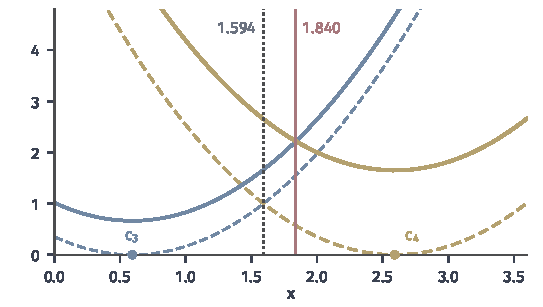
\includegraphics[width=92mm]{figures/07-probability/05-source-coding/matplotlib/quant-ecsq-threshold/figure.pdf}
 \caption{熵约束下的阈值。蓝色与黄色分别对应内侧重构值$c_3=0.594$（码长$1.328$ bit）与外侧重构值$c_4=2.594$（码长$3.299$ bit）。虚线为$(x-c_j)^{2}$，交于中点$1.594$；实线为$(x-c_j)^{2}+\lambda\ell(j)$，$\lambda=0.5$，交点右移到$1.840$（红线）。}
 \label{fig:quant-ecsq-threshold}
\end{BookInlineFigure}

阈值确定后，接着做两件事：把重构值移到新区间的质心，再把码长更新为新区间概率的理想码长。例中外侧区间概率降为$\mathrm{e}^{-1.840}/2=0.0794$，内侧升为$0.4206$；由式~\eqref{eq:quant-laplace-centroid}，新的质心为
\[
 c_3=0.6526,\qquad c_4=2.8400 .
\]
新的码长为$1.250$ bit与$3.655$ bit。平均失真升到$0.3608$，平均码长降到$1.631$ bit，目标$J_{0.5}$从$0.3524+0.5\times1.728=1.2165$降到$1.1765$。

这三步各自不增加$J_{\lambda}$。分配一步是对每个读数取带罚代价最小的区间，质心一步只改变失真项，理由与第~\ref{sec:quant-nonuniform}节相同。码长一步固定区间概率$p_j$，在$\sum_j2^{-\ell(j)}\leq1$下最小化$\sum_jp_j\ell(j)$；允许非整数码长时，上一章用KL散度的非负性证明了最小值在$\ell(j)=-\log_2p_j$取到，等于$H(J)$。实际码长必须是整数，理想码长只是这一步的近似，实际平均码长比它多不到一个比特，用块编码可以把这部分摊薄。

$\lambda$越大，外侧区间越被压缩，最终某些区间的概率可能趋于零，相当于自动减少了点数。在高分辨率下，可以说明熵约束量化的最优解接近均匀刻度，这与图~\ref{fig:quant-operational}中均匀量化加熵编码表现最好是一致的。总之，固定点数与固定平均码率是两种不同的约束，以平均码长为预算时，必须把它写进设计目标。
